% Options for packages loaded elsewhere
\PassOptionsToPackage{unicode}{hyperref}
\PassOptionsToPackage{hyphens}{url}
\PassOptionsToPackage{dvipsnames,svgnames,x11names}{xcolor}
%
\documentclass[
  letterpaper,
  DIV=11,
  numbers=noendperiod]{scrreprt}

\usepackage{amsmath,amssymb}
\usepackage{lmodern}
\usepackage{iftex}
\ifPDFTeX
  \usepackage[T1]{fontenc}
  \usepackage[utf8]{inputenc}
  \usepackage{textcomp} % provide euro and other symbols
\else % if luatex or xetex
  \usepackage{unicode-math}
  \defaultfontfeatures{Scale=MatchLowercase}
  \defaultfontfeatures[\rmfamily]{Ligatures=TeX,Scale=1}
\fi
% Use upquote if available, for straight quotes in verbatim environments
\IfFileExists{upquote.sty}{\usepackage{upquote}}{}
\IfFileExists{microtype.sty}{% use microtype if available
  \usepackage[]{microtype}
  \UseMicrotypeSet[protrusion]{basicmath} % disable protrusion for tt fonts
}{}
\makeatletter
\@ifundefined{KOMAClassName}{% if non-KOMA class
  \IfFileExists{parskip.sty}{%
    \usepackage{parskip}
  }{% else
    \setlength{\parindent}{0pt}
    \setlength{\parskip}{6pt plus 2pt minus 1pt}}
}{% if KOMA class
  \KOMAoptions{parskip=half}}
\makeatother
\usepackage{xcolor}
\setlength{\emergencystretch}{3em} % prevent overfull lines
\setcounter{secnumdepth}{5}
% Make \paragraph and \subparagraph free-standing
\ifx\paragraph\undefined\else
  \let\oldparagraph\paragraph
  \renewcommand{\paragraph}[1]{\oldparagraph{#1}\mbox{}}
\fi
\ifx\subparagraph\undefined\else
  \let\oldsubparagraph\subparagraph
  \renewcommand{\subparagraph}[1]{\oldsubparagraph{#1}\mbox{}}
\fi

\usepackage{color}
\usepackage{fancyvrb}
\newcommand{\VerbBar}{|}
\newcommand{\VERB}{\Verb[commandchars=\\\{\}]}
\DefineVerbatimEnvironment{Highlighting}{Verbatim}{commandchars=\\\{\}}
% Add ',fontsize=\small' for more characters per line
\usepackage{framed}
\definecolor{shadecolor}{RGB}{241,243,245}
\newenvironment{Shaded}{\begin{snugshade}}{\end{snugshade}}
\newcommand{\AlertTok}[1]{\textcolor[rgb]{0.68,0.00,0.00}{#1}}
\newcommand{\AnnotationTok}[1]{\textcolor[rgb]{0.37,0.37,0.37}{#1}}
\newcommand{\AttributeTok}[1]{\textcolor[rgb]{0.40,0.45,0.13}{#1}}
\newcommand{\BaseNTok}[1]{\textcolor[rgb]{0.68,0.00,0.00}{#1}}
\newcommand{\BuiltInTok}[1]{\textcolor[rgb]{0.00,0.23,0.31}{#1}}
\newcommand{\CharTok}[1]{\textcolor[rgb]{0.13,0.47,0.30}{#1}}
\newcommand{\CommentTok}[1]{\textcolor[rgb]{0.37,0.37,0.37}{#1}}
\newcommand{\CommentVarTok}[1]{\textcolor[rgb]{0.37,0.37,0.37}{\textit{#1}}}
\newcommand{\ConstantTok}[1]{\textcolor[rgb]{0.56,0.35,0.01}{#1}}
\newcommand{\ControlFlowTok}[1]{\textcolor[rgb]{0.00,0.23,0.31}{#1}}
\newcommand{\DataTypeTok}[1]{\textcolor[rgb]{0.68,0.00,0.00}{#1}}
\newcommand{\DecValTok}[1]{\textcolor[rgb]{0.68,0.00,0.00}{#1}}
\newcommand{\DocumentationTok}[1]{\textcolor[rgb]{0.37,0.37,0.37}{\textit{#1}}}
\newcommand{\ErrorTok}[1]{\textcolor[rgb]{0.68,0.00,0.00}{#1}}
\newcommand{\ExtensionTok}[1]{\textcolor[rgb]{0.00,0.23,0.31}{#1}}
\newcommand{\FloatTok}[1]{\textcolor[rgb]{0.68,0.00,0.00}{#1}}
\newcommand{\FunctionTok}[1]{\textcolor[rgb]{0.28,0.35,0.67}{#1}}
\newcommand{\ImportTok}[1]{\textcolor[rgb]{0.00,0.46,0.62}{#1}}
\newcommand{\InformationTok}[1]{\textcolor[rgb]{0.37,0.37,0.37}{#1}}
\newcommand{\KeywordTok}[1]{\textcolor[rgb]{0.00,0.23,0.31}{#1}}
\newcommand{\NormalTok}[1]{\textcolor[rgb]{0.00,0.23,0.31}{#1}}
\newcommand{\OperatorTok}[1]{\textcolor[rgb]{0.37,0.37,0.37}{#1}}
\newcommand{\OtherTok}[1]{\textcolor[rgb]{0.00,0.23,0.31}{#1}}
\newcommand{\PreprocessorTok}[1]{\textcolor[rgb]{0.68,0.00,0.00}{#1}}
\newcommand{\RegionMarkerTok}[1]{\textcolor[rgb]{0.00,0.23,0.31}{#1}}
\newcommand{\SpecialCharTok}[1]{\textcolor[rgb]{0.37,0.37,0.37}{#1}}
\newcommand{\SpecialStringTok}[1]{\textcolor[rgb]{0.13,0.47,0.30}{#1}}
\newcommand{\StringTok}[1]{\textcolor[rgb]{0.13,0.47,0.30}{#1}}
\newcommand{\VariableTok}[1]{\textcolor[rgb]{0.07,0.07,0.07}{#1}}
\newcommand{\VerbatimStringTok}[1]{\textcolor[rgb]{0.13,0.47,0.30}{#1}}
\newcommand{\WarningTok}[1]{\textcolor[rgb]{0.37,0.37,0.37}{\textit{#1}}}

\providecommand{\tightlist}{%
  \setlength{\itemsep}{0pt}\setlength{\parskip}{0pt}}\usepackage{longtable,booktabs,array}
\usepackage{calc} % for calculating minipage widths
% Correct order of tables after \paragraph or \subparagraph
\usepackage{etoolbox}
\makeatletter
\patchcmd\longtable{\par}{\if@noskipsec\mbox{}\fi\par}{}{}
\makeatother
% Allow footnotes in longtable head/foot
\IfFileExists{footnotehyper.sty}{\usepackage{footnotehyper}}{\usepackage{footnote}}
\makesavenoteenv{longtable}
\usepackage{graphicx}
\makeatletter
\def\maxwidth{\ifdim\Gin@nat@width>\linewidth\linewidth\else\Gin@nat@width\fi}
\def\maxheight{\ifdim\Gin@nat@height>\textheight\textheight\else\Gin@nat@height\fi}
\makeatother
% Scale images if necessary, so that they will not overflow the page
% margins by default, and it is still possible to overwrite the defaults
% using explicit options in \includegraphics[width, height, ...]{}
\setkeys{Gin}{width=\maxwidth,height=\maxheight,keepaspectratio}
% Set default figure placement to htbp
\makeatletter
\def\fps@figure{htbp}
\makeatother

\KOMAoption{captions}{tableheading}
\makeatletter
\makeatother
\makeatletter
\@ifpackageloaded{bookmark}{}{\usepackage{bookmark}}
\makeatother
\makeatletter
\@ifpackageloaded{caption}{}{\usepackage{caption}}
\AtBeginDocument{%
\ifdefined\contentsname
  \renewcommand*\contentsname{Table of contents}
\else
  \newcommand\contentsname{Table of contents}
\fi
\ifdefined\listfigurename
  \renewcommand*\listfigurename{List of Figures}
\else
  \newcommand\listfigurename{List of Figures}
\fi
\ifdefined\listtablename
  \renewcommand*\listtablename{List of Tables}
\else
  \newcommand\listtablename{List of Tables}
\fi
\ifdefined\figurename
  \renewcommand*\figurename{Figure}
\else
  \newcommand\figurename{Figure}
\fi
\ifdefined\tablename
  \renewcommand*\tablename{Table}
\else
  \newcommand\tablename{Table}
\fi
}
\@ifpackageloaded{float}{}{\usepackage{float}}
\floatstyle{ruled}
\@ifundefined{c@chapter}{\newfloat{codelisting}{h}{lop}}{\newfloat{codelisting}{h}{lop}[chapter]}
\floatname{codelisting}{Listing}
\newcommand*\listoflistings{\listof{codelisting}{List of Listings}}
\makeatother
\makeatletter
\@ifpackageloaded{caption}{}{\usepackage{caption}}
\@ifpackageloaded{subcaption}{}{\usepackage{subcaption}}
\makeatother
\makeatletter
\@ifpackageloaded{tcolorbox}{}{\usepackage[many]{tcolorbox}}
\makeatother
\makeatletter
\@ifundefined{shadecolor}{\definecolor{shadecolor}{rgb}{.97, .97, .97}}
\makeatother
\makeatletter
\makeatother
\ifLuaTeX
  \usepackage{selnolig}  % disable illegal ligatures
\fi
\IfFileExists{bookmark.sty}{\usepackage{bookmark}}{\usepackage{hyperref}}
\IfFileExists{xurl.sty}{\usepackage{xurl}}{} % add URL line breaks if available
\urlstyle{same} % disable monospaced font for URLs
\hypersetup{
  pdftitle={Ramble On's Progress Journal},
  colorlinks=true,
  linkcolor={blue},
  filecolor={Maroon},
  citecolor={Blue},
  urlcolor={Blue},
  pdfcreator={LaTeX via pandoc}}

\title{Ramble On's Progress Journal}
\author{}
\date{}

\begin{document}
\maketitle
\ifdefined\Shaded\renewenvironment{Shaded}{\begin{tcolorbox}[frame hidden, sharp corners, interior hidden, borderline west={3pt}{0pt}{shadecolor}, enhanced, boxrule=0pt, breakable]}{\end{tcolorbox}}\fi

\renewcommand*\contentsname{Table of contents}
{
\hypersetup{linkcolor=}
\setcounter{tocdepth}{2}
\tableofcontents
}
\bookmarksetup{startatroot}

\hypertarget{introduction}{%
\chapter*{Introduction}\label{introduction}}
\addcontentsline{toc}{chapter}{Introduction}

This progress journal covers Ramble On's work during their term at
\href{https://mef-bda503.github.io/fall22/}{BDA 503 Fall 2022}.

Each section is an assignment or an individual work.

\bookmarksetup{startatroot}

\hypertarget{assignment-1}{%
\chapter{Assignment 1}\label{assignment-1}}

First, the necessary libraries and data are imported.

\begin{Shaded}
\begin{Highlighting}[]
\CommentTok{\# install.packages("readxl")}
\CommentTok{\# install.package(kni)}
\FunctionTok{library}\NormalTok{(readxl)}
\FunctionTok{library}\NormalTok{(knitr)}
\FunctionTok{library}\NormalTok{(ggplot2)}
\FunctionTok{library}\NormalTok{(dplyr)}
\FunctionTok{library}\NormalTok{(scales)}
\NormalTok{df }\OtherTok{\textless{}{-}}\NormalTok{ readxl}\SpecialCharTok{::}\FunctionTok{read\_excel}\NormalTok{(}\StringTok{"assignment1/startup\_deals\_2021.xlsx"}\NormalTok{)}
\end{Highlighting}
\end{Shaded}

The problematic characters in the column names are removed to make
accessing the columns easier. Then we can get a ``glimpse'' of our data.

\begin{Shaded}
\begin{Highlighting}[]
\FunctionTok{names}\NormalTok{(df) }\OtherTok{\textless{}{-}} \FunctionTok{gsub}\NormalTok{(}\StringTok{"\%"}\NormalTok{, }\StringTok{""}\NormalTok{, }\FunctionTok{names}\NormalTok{(df))}
\FunctionTok{names}\NormalTok{(df) }\OtherTok{\textless{}{-}} \FunctionTok{gsub}\NormalTok{(}\StringTok{" "}\NormalTok{, }\StringTok{"\_"}\NormalTok{, }\FunctionTok{names}\NormalTok{(df))}
\FunctionTok{names}\NormalTok{(df) }\OtherTok{\textless{}{-}} \FunctionTok{gsub}\NormalTok{(}\StringTok{"[()]"}\NormalTok{, }\StringTok{""}\NormalTok{, }\FunctionTok{names}\NormalTok{(df))}
\FunctionTok{glimpse}\NormalTok{(df)}
\end{Highlighting}
\end{Shaded}

\begin{verbatim}
Rows: 297
Columns: 9
$ Target_Company      <chr> "Abonesepeti", "Abrakadabra", "Ace Games", "Adlema~
$ Sector              <chr> "SaaS", "Gaming", "Gaming", "Internet of things", ~
$ Investor            <chr> "Keiretsu Forum, Berkan Burla", "WePlay Ventures",~
$ Announcement_Date   <chr> "June 2021", "December 2021", "April 2021", "June ~
$ Financial_Investor  <chr> "Yes", "Yes", "Yes", "Yes", "Yes", "Yes", "Yes", "~
$ `Investor's_Origin` <chr> "Turkey", "Turkey", "Turkey, USA", "Turkey", "Turk~
$ Stake_              <chr> "5.00%", "5.00%", "NA", "NA", "NA", "NA", "10.92%"~
$ Deal_Value_USD      <chr> "100000", "250000", "NA", "120000", "100000", "100~
$ Investment_Stage    <chr> "Seed Stage", "Seed Stage", "Seed Stage", "Seed St~
\end{verbatim}

It can be seen that the ``Stake\_'' and ``Deal\_Value\_USD'' columns
appear as strings. That's not good for business.

Let's start with the ``Deal\_Value\_USD'' column. suppressWarnings used
to avoid the warnings for the NaN values.

\begin{Shaded}
\begin{Highlighting}[]
\NormalTok{df}\SpecialCharTok{$}\StringTok{"Deal\_Value\_USD"}\OtherTok{\textless{}{-}} \FunctionTok{suppressWarnings}\NormalTok{(}\FunctionTok{as.integer}\NormalTok{(df}\SpecialCharTok{$}\StringTok{"Deal\_Value\_USD"}\NormalTok{))}
\end{Highlighting}
\end{Shaded}

It gets a bit cumbersome when it comes to the ``Stake\_'' column. If we
were to change it like we did for the first column, we would get NaNs
for the values. We can check the values in the column to investigate
this problem.

\begin{Shaded}
\begin{Highlighting}[]
\FunctionTok{table}\NormalTok{(df[}\StringTok{"Stake\_"}\NormalTok{])}
\end{Highlighting}
\end{Shaded}

\begin{verbatim}
Stake_
  0.46%   1.33%  10.00%  10.42%  10.65% 10.71 % 10.91 %  10.92% 100.00%  11.00% 
      1       1      12       1       1       1       1       1      12       2 
 11.03% 11.11 %  11.55%  12.00%  12.50% 12.61 %  14.06%  14.28%  14.29%  14.30% 
      1       1       1       1       4       1       1       1       2       1 
 14.60% 14.71 % 14.91 %  15.00%  15.38%  15.49%  15.50%  15.60%  15.79%  16.13% 
      1       1       1       1       1       1       1       1       1       2 
  1750%  18.66%  19.99%   2.00%  2.21 %   2.59%  20.00%  20.83%  22.00%  22.73% 
      1       1       1       2       1       1       7       1       1       1 
 23.50%  24.29%  25.00%  25.23%  28.00%   3.33%   3.38%   3.63%  30.00%  33.33% 
      1       1       2       1       1       2       1       1       1       1 
 35.00%  35.09%  37.50%  37.70%   4.00%   4.44%   4.75%   5.00%   5.20%   5.67% 
      1       1       1       1       1       1       1      10       1       1 
 5.81 %   5.88%   5.90%  50.00%   6.00%   6.25%   6.34%  6.51 %   6.60%  60.00% 
      1       2       1       3       2       1       1       1       1       4 
 69.82%   7.00%   7.14%   7.39%   7.50%   7.69%  75.00%   8.05%   8.08%   8.33% 
      1       1       1       1       1       1       1       1       1       1 
  8.47%   8.70%  88.89%   9.39%   9.40%  9.91 %      NA 
      2       1       1       1       1       1     157 
\end{verbatim}

``\%'' characters and the white space in some of the cells cause
problems. They are removed, and the type is changed. The warnings are
suppressed again.

\begin{Shaded}
\begin{Highlighting}[]
\NormalTok{df}\SpecialCharTok{$}\StringTok{"Stake\_"}\OtherTok{\textless{}{-}} \FunctionTok{gsub}\NormalTok{(}\StringTok{"\%"}\NormalTok{,}\StringTok{""}\NormalTok{, df}\SpecialCharTok{$}\StringTok{"Stake\_"}\NormalTok{) }\SpecialCharTok{\%\textgreater{}\%} \FunctionTok{trimws}\NormalTok{(df}\SpecialCharTok{$}\StringTok{"Stake\_"}\NormalTok{, }\AttributeTok{which =} \FunctionTok{c}\NormalTok{(}\StringTok{"both"}\NormalTok{)) }\SpecialCharTok{\%\textgreater{}\%} \FunctionTok{as.numeric}\NormalTok{(df}\SpecialCharTok{$}\StringTok{"Stake\_"}\NormalTok{)}
\FunctionTok{glimpse}\NormalTok{(df)}
\end{Highlighting}
\end{Shaded}

\begin{verbatim}
Rows: 297
Columns: 9
$ Target_Company      <chr> "Abonesepeti", "Abrakadabra", "Ace Games", "Adlema~
$ Sector              <chr> "SaaS", "Gaming", "Gaming", "Internet of things", ~
$ Investor            <chr> "Keiretsu Forum, Berkan Burla", "WePlay Ventures",~
$ Announcement_Date   <chr> "June 2021", "December 2021", "April 2021", "June ~
$ Financial_Investor  <chr> "Yes", "Yes", "Yes", "Yes", "Yes", "Yes", "Yes", "~
$ `Investor's_Origin` <chr> "Turkey", "Turkey", "Turkey, USA", "Turkey", "Turk~
$ Stake_              <dbl> 5.00, 5.00, NA, NA, NA, NA, 10.92, NA, NA, 15.38, ~
$ Deal_Value_USD      <int> 100000, 250000, NA, 120000, 100000, 1000000, 25000~
$ Investment_Stage    <chr> "Seed Stage", "Seed Stage", "Seed Stage", "Seed St~
\end{verbatim}

\hypertarget{value-by-company}{%
\section{Value by Company}\label{value-by-company}}

The amount of investment received by companies can be examined as the
first analysis. To do so, we should group the data set by company name
and sum the deal values.

\begin{Shaded}
\begin{Highlighting}[]
\NormalTok{df\_grouped }\OtherTok{\textless{}{-}}\NormalTok{ df }\SpecialCharTok{\%\textgreater{}\%}
  \FunctionTok{group\_by}\NormalTok{(Target\_Company) }\SpecialCharTok{\%\textgreater{}\%}
  \FunctionTok{summarize}\NormalTok{(}\AttributeTok{Deal\_Value\_USD =} \FunctionTok{sum}\NormalTok{(Deal\_Value\_USD)) }\SpecialCharTok{\%\textgreater{}\%}
  \FunctionTok{arrange}\NormalTok{(}\FunctionTok{desc}\NormalTok{(Deal\_Value\_USD))}

\FunctionTok{kable}\NormalTok{(}\FunctionTok{head}\NormalTok{(df\_grouped, }\DecValTok{10}\NormalTok{))}
\end{Highlighting}
\end{Shaded}

\begin{longtable}[]{@{}lr@{}}
\toprule()
Target\_Company & Deal\_Value\_USD \\
\midrule()
\endhead
trendyol & 1435000000 \\
Getir & 1018000000 \\
hepsiburada & 761481000 \\
Dream Games & 155000050 \\
Libra Softworks & 30000000 \\
Prota & 30000000 \\
BluTV & 20800000 \\
Arvento & 20565000 \\
Akinon & 20000000 \\
Biotrend Energy & 20000000 \\
\bottomrule()
\end{longtable}

We can also visualize these companies and compare them.

Visualizing so many companies will make the plot unreadable. We can just
select the top 5\% and feed them to our plot.

We first calculate the value for the filter, then add it to the code,
and then we sort the bars according to the values. Next, we insert the
elements of the plot.

\begin{Shaded}
\begin{Highlighting}[]
\NormalTok{qu }\OtherTok{\textless{}{-}} \FunctionTok{quantile}\NormalTok{(df\_grouped}\SpecialCharTok{$}\NormalTok{Deal\_Value\_USD, }\AttributeTok{probs =} \FloatTok{0.95}\NormalTok{, }\AttributeTok{na.rm =} \ConstantTok{TRUE}\NormalTok{)}

\NormalTok{df\_grouped }\SpecialCharTok{\%\textgreater{}\%} \FunctionTok{filter}\NormalTok{(Deal\_Value\_USD }\SpecialCharTok{\textgreater{}=}\NormalTok{ qu) }\SpecialCharTok{\%\textgreater{}\%}
  \FunctionTok{ggplot}\NormalTok{(}\FunctionTok{aes}\NormalTok{(}\AttributeTok{x =} \FunctionTok{reorder}\NormalTok{(Target\_Company, }\SpecialCharTok{+}\NormalTok{Deal\_Value\_USD),}\AttributeTok{y =}\NormalTok{ Deal\_Value\_USD))}\SpecialCharTok{+}     
  \FunctionTok{geom\_col}\NormalTok{(}\AttributeTok{width =} \FloatTok{0.5}\NormalTok{) }\SpecialCharTok{+} \FunctionTok{theme}\NormalTok{(}\AttributeTok{axis.text.x =} \FunctionTok{element\_text}\NormalTok{(}\AttributeTok{angle =} \DecValTok{45}\NormalTok{, }\AttributeTok{hjust=}\DecValTok{1}\NormalTok{)) }\SpecialCharTok{+} 
  \FunctionTok{ggtitle}\NormalTok{(}\StringTok{"Total Investments by Company"}\NormalTok{) }\SpecialCharTok{+}
  \FunctionTok{xlab}\NormalTok{(}\StringTok{"Company"}\NormalTok{) }\SpecialCharTok{+} \FunctionTok{ylab}\NormalTok{(}\StringTok{"Deal Value in USD (Millions)"}\NormalTok{) }\SpecialCharTok{+} 
  \FunctionTok{scale\_y\_continuous}\NormalTok{(}\AttributeTok{labels =} \FunctionTok{label\_number}\NormalTok{(}\AttributeTok{suffix =} \StringTok{" M"}\NormalTok{, }\AttributeTok{scale =} \FloatTok{1e{-}6}\NormalTok{))}
\end{Highlighting}
\end{Shaded}

\begin{figure}[H]

{\centering 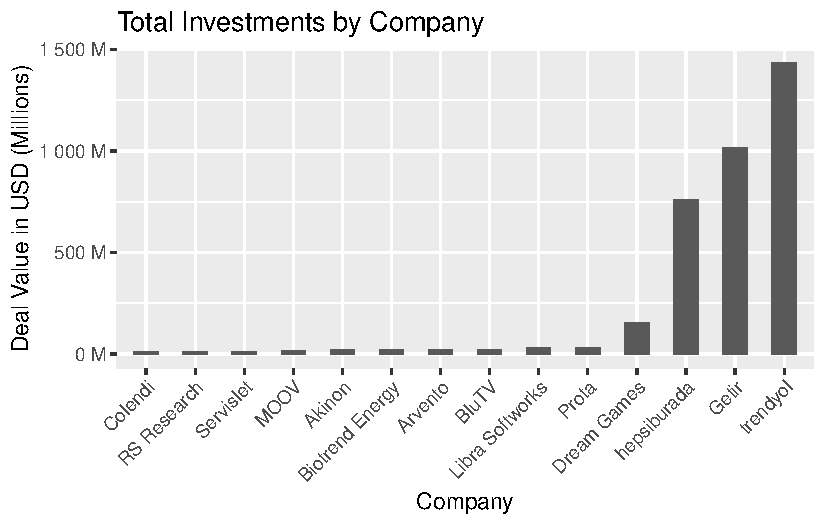
\includegraphics{./assignment1_files/figure-pdf/unnamed-chunk-5-1.pdf}

}

\end{figure}



\end{document}
